%set the master document for easy compilation
%!TEX root = ../D3_5_2.tex

%-----------------------------------------------------------------------
\section{Manage Radio Communication}
%-----------------------------------------------------------------------
%\tbc
%Group4 (Uwe Steinke)

\subsection{Management of Radio Communication (\emph{MoRC})} 

\subsubsection{Reference to the SRS}
The management of radio communication is specified in Subset-026, chap. 3.5. 

\subsubsection{Short description of the functionality}

The management of radio communication \textit{MoRC} implements the on board management part of a single communication session with the track, i.e. a single RBC. It controls the establishing, maintaining and termination process of a radio communication session and steers the underlying communication safety layer and the mobile device. Those and the data transfer itself are not part of the function. 

\subsubsection{Interface}

\paragraph{Inputs}
The MoRC function takes as inputs datagrams received from track, OBU internal phases and status information and configuration data: 

\begin{itemize}
 \item Datagrams received from track (\textit{inMessage}):
 \begin{itemize}
  \item Packet 42 (session management) received from balise group or RBC
  \item Packet 45 (radio network registration) received from balise group or RBC
  \item Message 32 (RBC/RIU System Version) received from RBC: \textit{MoRC} only needs to know if the system version received from track side is supported by the OBU.
  \item Message 38 (initiation of a communication session) received from RBC
  \item Message 39 (acknowledgement of termination of a communication session)
 \end{itemize}

 \item \textit{obuEventsAndPhases}: information about OBU internal events and OBU internal phases:

  \begin{itemize}
   \item \textit{atPowerDown}
   \item \textit{atPowerUp}
   \item \textit{atStartOfMission}
   \item \textit{startOfMissionProcedureIsGoingOn}
   \item \textit{startOfMissionProcedureCompleted}
   \item \textit{trainIsRejectedByRBC\_duringStartOfMission}
   \item \textit{endOfMissionIsExecuted}
   \item \textit{driverClosesTheDeskduringStartOfMission}
   \item \textit{driverHasManuallyChangedLevel}
   \item \textit{afterDriverEntryOfANewRadioNetworkID}
   \item \textit{triggerDecisionThatNoRadioNetworkIDAvailable}
   \item \textit{isPartOfAnOngoingStartOfMissionProcedure}
   \item \textit{trainPassesALevelTransitionBorder}
   \item \textit{trainPassesA\_RBC\_RBC\_border\_WithItsFrontEnd}
   \item \textit{trainExitedFromAnRBCArea}
   \item \textit{modeChangeHasToBeReportedToRBC}
   \item \textit{trainFrontInsideInAnAnnouncedRadioHole}
   \item \textit{trainFrontReachesEndOfAnnouncedRadioHole}
   \item \textit{OBU\_hasToEstablishANewSession}
   \item \textit{isInCommunicationSessionWithAnRIU}
   \item \textit{errorConditionRequiringTerminationDetected}
  \end{itemize}

  \item Current OBU internal states:
  
  \begin{itemize}
   \item \textit{currentTime}: current OBU system time
   \item \textit{t\_train}: current trainborne clock (T\_TRAIN) as specified in Subset-026, chap. 7
   \item \textit{mode}: current OBU mode
   \item \textit{level}: current OBU level
  \end{itemize}

  \item \textit{statusOfMobile}: status of the associated mobile device
  
  \item configuration parameters:
  
   \begin{itemize}
    \item \textit{onboardPhoneNumbers} (NID\_RADIO)
    \item \textit{radioNetworkIDs}: Identities of radio networks (NID\_MN): default, memorized or from driver  
    \item \textit{nid\_engine}: Onboard ETCS identity (NID\_ENGINE)
    \item \textit{connectionStatusTimerInterval}: Connection status timer period 
   \end{itemize} 

 \end{itemize} 

\paragraph{Outputs}

MoRC generates a couple of outputs: 

\begin{itemize}
 \item \textit{MessageToRBC}: messages to be sent to the RBC: 

  \begin{itemize}
   \item Message 155 (initiation of a communication session)
   \item Message 156 (termination of a communication session)
   \item Message 159 (session established)
   \item Message 154 (no compatible version supported) 
  \end{itemize}

 \item Action triggers: 
 
  \begin{itemize}
   \item \textit{sendAPositionReport}: triggers a position report to be sent to the RBC
   \item \textit{memorizeTheLastRadioNetworkID}: triggers to store the last radio network ID for later use
   \item \textit{orderTheRegistrationOfItsConnectedMobiles}
   \item \textit{rejectOrderToContactRBC\_or\_RIU}
   \item \textit{InformTheDriverThatNoConnectionWasSetup}
   \item \textit{requestTheSetupOfASafeRadioConnection}: initiate the setup of a safe radio connection
   \item \textit{requestReleaseOfSafeRadioConnectionWithTrackside}: initiate the release of a safe radio connection
   \item \textit{ignoreMessagesFromRBC\_except\_m39\_AckOfTerminationOfCommunicationSession}
   \item \textit{sessionSuccessfullyEstablished}
  \end{itemize} 

 \item \textit{cmdsToMobile}: control commands to the mobile device
 
 \item Status information: 
 
  \begin{itemize}
   \item \textit{sessionStatus}: current session status
   \item \textit{mobileSWStatus}: connection status
   \item \textit{currentRadioNetworkID}: current radio network ID
  \end{itemize}
 
\end{itemize}

\begin{figure}
\centering
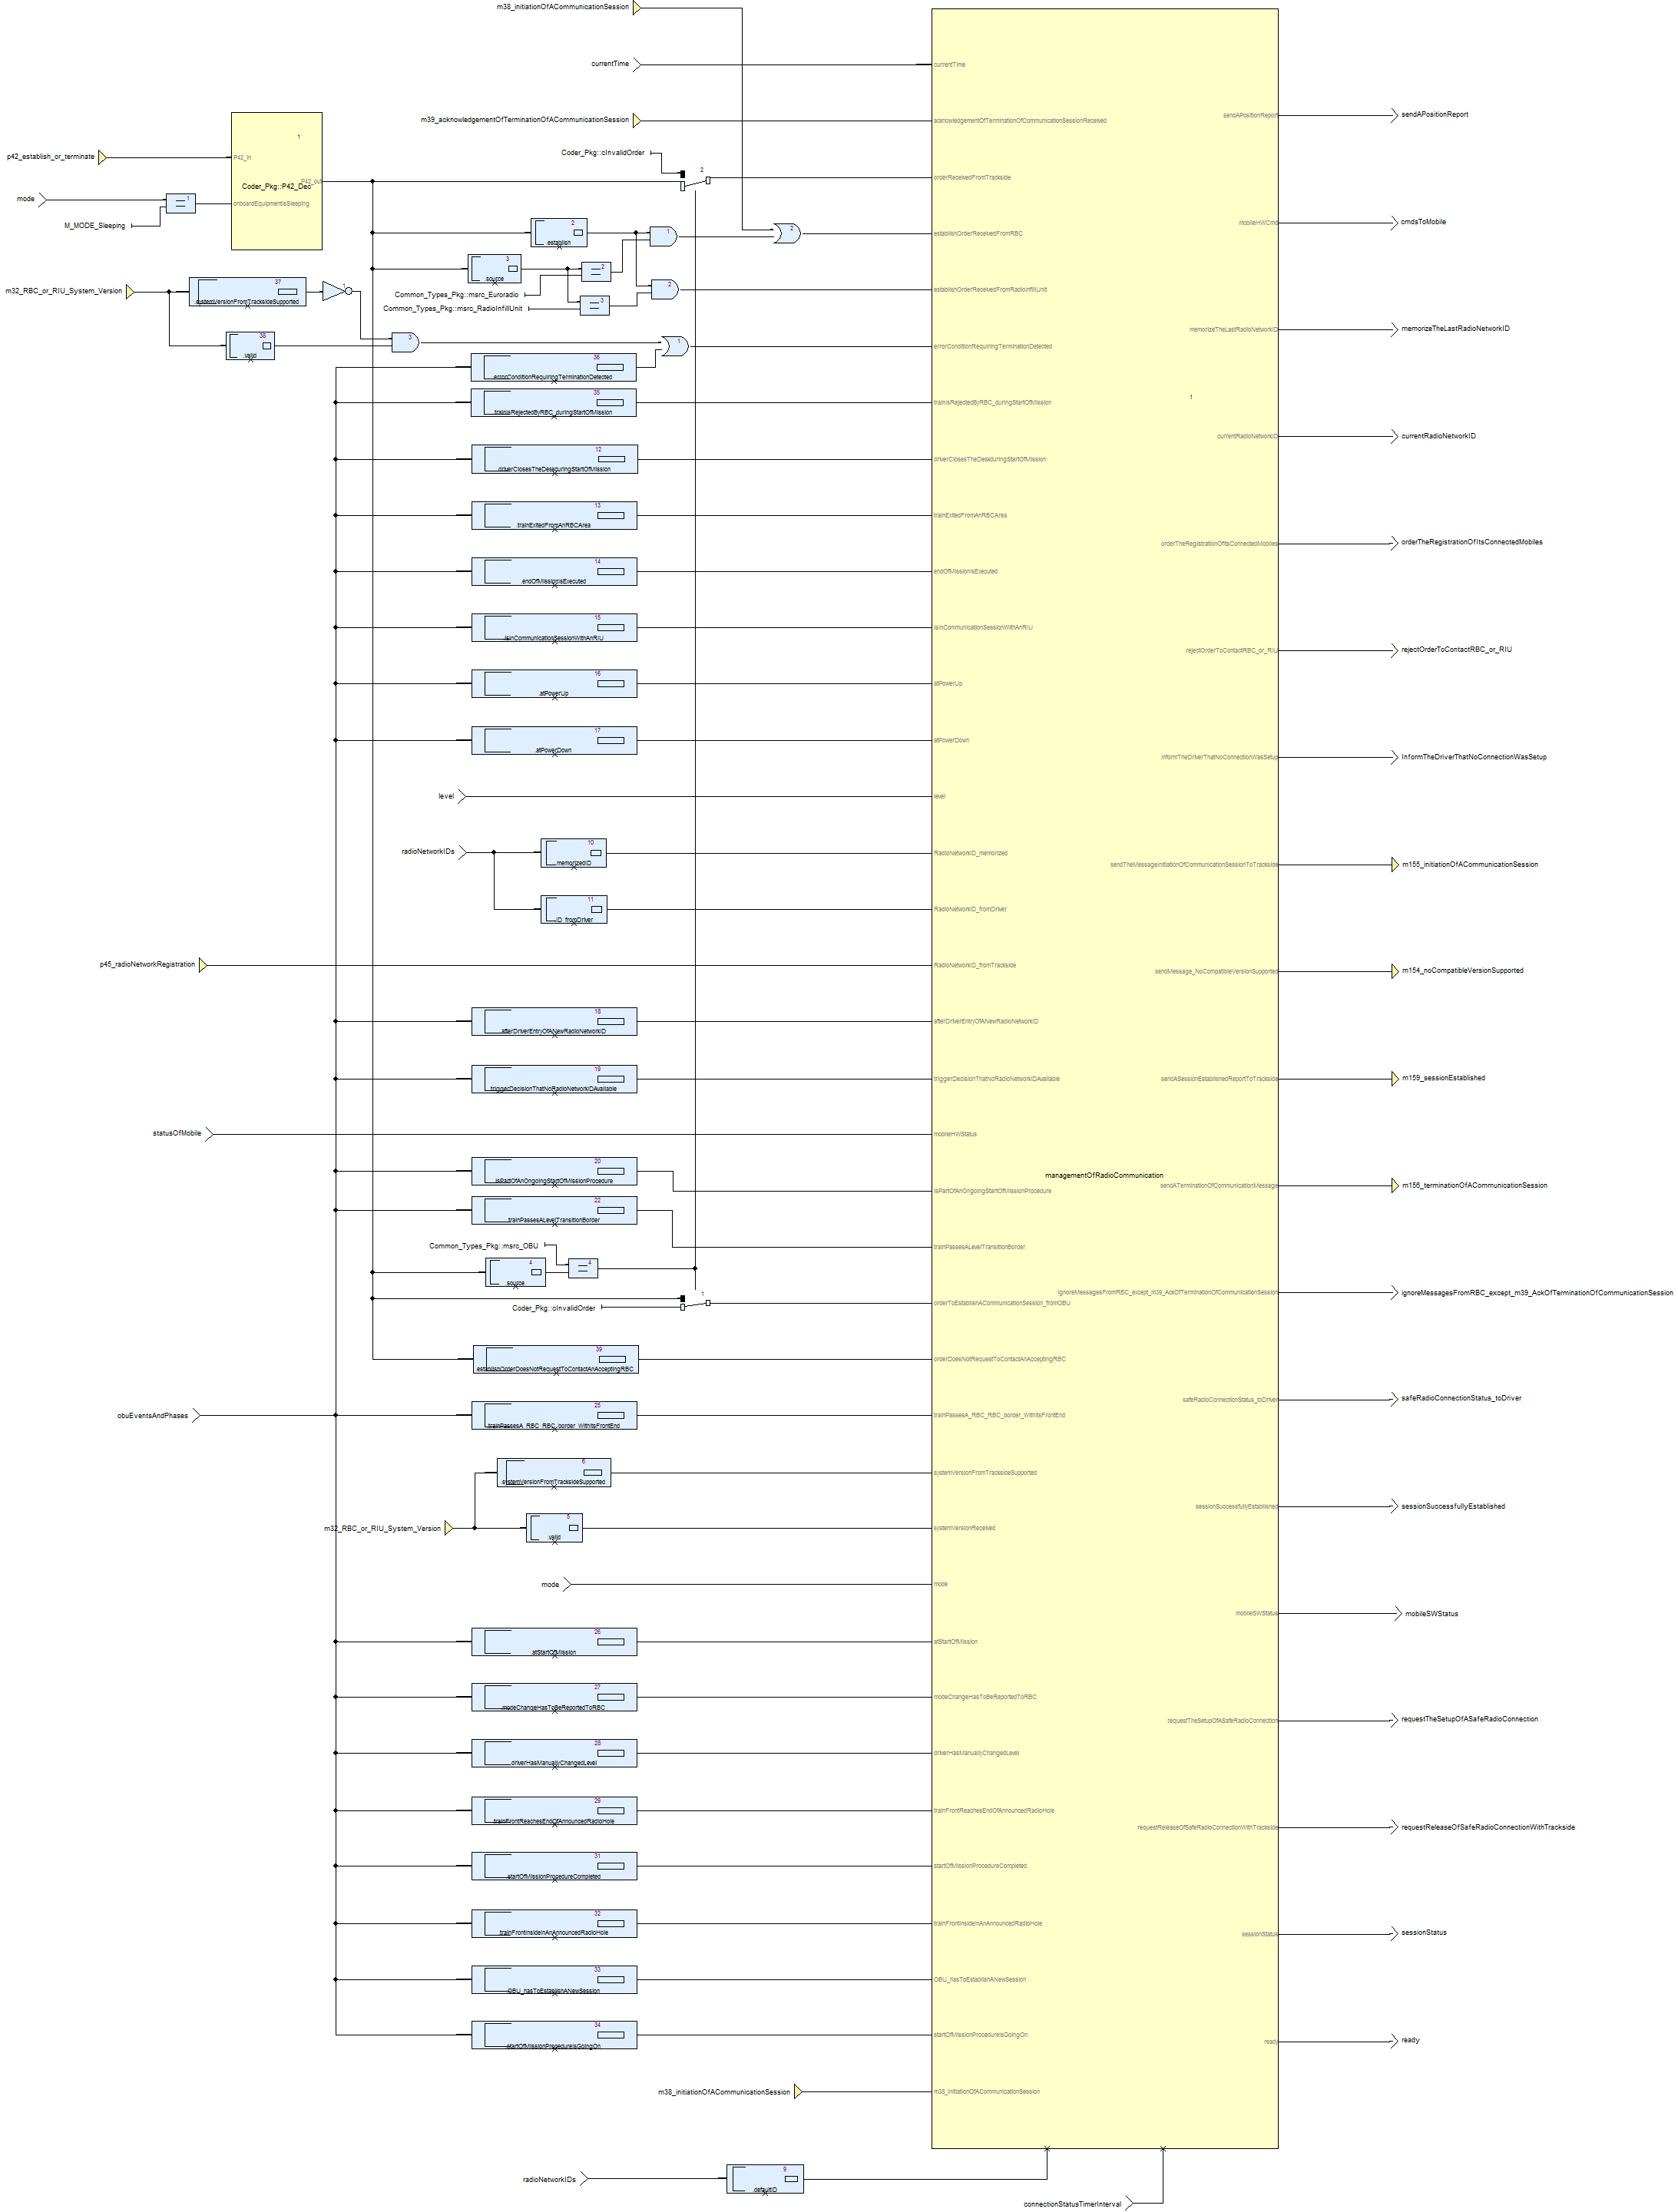
\includegraphics[scale=0.2]{../images/MoRC_Main.png}
\caption{Main function of \textit{MoRC}.}
\end{figure}

\begin{figure}
\centering
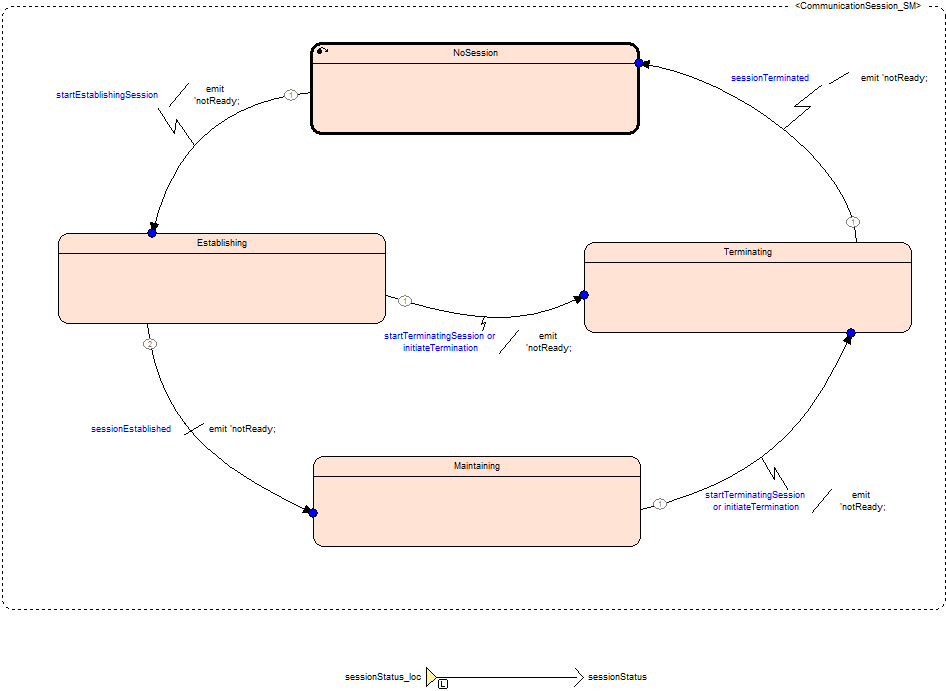
\includegraphics[width=\textwidth]{../images/MoRC_SessionManagement.png}
\caption{Implementation of session states.}
\end{figure}


\subsubsection{Functional Design Description}

The kernel function of the \textit{MoRC} component is \emph{managementOfRadioCommunication} (figure ???). The implementation is kept close to the prose of Subset-026, chap. 3.5. Since chap. 3.5 rarely refers to terms, variable types, packets and messages of the ETCS language as specified in Subset-026, chap. 7 and 8, \emph{managementOfRadioCommunication} does neither. 

To be capable of being integrated with other OBU software components, \emph{MoRC} had to be wrapped with a transformer between the ETCS and the "chap. 3.5" language. This is the purpose of the main function of \emph{MoRC}, \emph{MoRC\_Main}. 



The function \emph{managementOfRadioCommunication} implements the session states establishing, maintaining and termination as described in Subset-026, chap. 3.5. A SCADE state machine reflects this state model (figure ???) accurately. Within each of the states, the activities needed as long as the state is active, are performed. When there is no communication session (state \emph{NoSession}) currently, the state machine waits for events that initiate a session (subfunction \emph{initiate\_a\_Session}). When the appropriate conditions are fulfilled, the state machine moves to the \textit{Establishing} state. Here in, it runs through the sequence required fore establishing a session (subfunction \emph{establish\_a\_Session}. Dependent on the results, the state machine changes over to the \emph{Maintaining} or \emph{Terminating} state. While in \emph{Maintaining}, the communication connection is monitored. When an event triggering the session termination occurs, the state machine switches to the state \emph{Terminating} with the subfunction \emph{terminating\_a\_CommunicationSession} and performs the session termination sequence. 

In parallel to the main state machine, \emph{managementOfRadioCommunication} monitors all the time whether the session has to be terminated (subfunction \emph{initiateTerminatingASession}) or if the session has the be terminated and subsequently established (subfunction \emph{terminateAndEstablishSession}). \emph{registeringToTheRadioNetwork} is responsible for connection to the radio network. \emph{safeRadioConnectionIndication} controls the radio connection indication for the driver.


\subsubsection{Reference to the Scade Model}

The MoRC SCADE model resides at \url{https://github.com/openETCS/modeling/tree/master/model/Scade/System/ObuFunctions/Radio/MoRC} .






